\documentclass{standalone}

\usepackage[]{tikz}
\usepackage{pgfplots}
\usetikzlibrary{positioning, calc, patterns}

\begin{document}

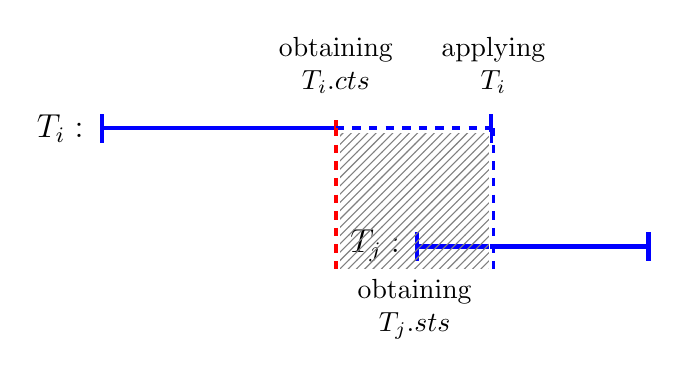
\begin{tikzpicture}[txt/.style = {align = center}]

\def\dist{0.8}

% T_i
\node[font = \large] at (-0.5, 0) {$T_i:$};

\draw[ultra thick, blue, |-] (0,0) to (3,0);
\draw[ultra thick, red] (3,0.1) to (3, 0);
\node[txt] at (3, \dist) {obtaining \\ $T_i.cts$};

\draw[ultra thick, dashed, blue, -|] (3,0) to (5,0);
\node[txt] at (5, \dist) {applying \\ $T_i$};

\draw[very thick, red, dashed] (3,0) to (3, -1.8);
\draw[very thick, blue, dashed] (5,0) to (5, -1.8);

% T_j
\node[font = \large] at (3.5, -1.5) {$T_j:$};
\draw[ultra thick, blue, |-|] (4,-1.5) to (7,-1.5);
\node[txt] at (4, -2.3) {obtaining \\ $T_j.sts$};

% forbidden
\draw[color = white, pattern color = gray, pattern = north east lines] (3.05,-0.05) rectangle (4.95,-1.8);

\end{tikzpicture}
\end{document}
